\documentclass{article}
\usepackage{times}
\usepackage{graphicx}
\usepackage{subfigure} 
\usepackage{natbib}
\usepackage{algorithm}
\usepackage{algorithmic}
\usepackage{amsmath}
\usepackage{hyperref}
\newcommand{\theHalgorithm}{\arabic{algorithm}}
%\usepackage{icml2015stylefiles/icml2015} 
\usepackage[accepted]{icml2015stylefiles/icml2015}


\newcommand{\vx}{\mathbf{x}}
\newcommand{\vv}{\mathbf{v}}
\newcommand{\vg}{\mathbf{g}}
\newcommand{\vzero}{\mathbf{0}}
\newcommand{\ones}[1]{\mat{1}_{#1}}
\newcommand{\eye}[1]{\mat{E}_{#1}}
\newcommand{\tra}{^{\mathsf{T}}}

\newcommand{\numhypers}{N}
\newcommand{\numsteps}{T}
\newcommand{\drag}{\gamma}
\newcommand{\stepsize}{\alpha}

\newcommand\ourtitle{Gradient-based Hyperparameter Optimization through Reversible Learning}
% A short form for the running title is supplied here:
\icmltitlerunning{\ourtitle}

\begin{document} 

\twocolumn[
\icmltitle{\ourtitle}

% It is OKAY to include author information, even for blind
% submissions: the style file will automatically remove it for you
% unless you've provided the [accepted] option to the icml2015
% package.
\icmlauthor{Dougal Maclaurin}{maclaurin@physics.harvard.edu}
%\icmladdress{Harvard University, Cambridge, Massachusetts}
\icmlauthor{David Duvenaud}{dduvenaud@seas.harvard.edu}
%\icmladdress{Harvard University, Cambridge, Massachusetts}
\icmlauthor{Ryan P. Adams}{rpa@seas.harvard.edu}
%\icmladdress{Harvard University, Cambridge, Massachusetts}

% You may provide any keywords that you 
% find helpful for describing your paper; these are used to populate 
% the "keywords" metadata in the PDF but will not be shown in the document
\icmlkeywords{hyperparameters, neural networks, reversible computation, automatic differentiation, machine learning, ICML}

\vskip 0.3in
]

\begin{abstract} 
Tuning more than a small number of hyper parameters remains difficult due to the fact that gradients are typically unavailable.
We compute gradients of the cross-validation objective w.r.t. hyperparameters by chaining derivatives through the \emph{entire training procedure}, including hundreds of iterations of back propagation.
These gradients allows us to richly parameterize our learning procedures, optimizing complex learning rate schedules, weight initialization distributions, and neural net architectures.
We show state-of-the art results?
Our results also provide examples of optimal learning schedules and initialization strategies for several benchmark problems.
\end{abstract} 

\section{Introduction}
\label{intro}



\section{Meta-Optimization}

The current state-of-the-art for hyperparameter optimization is achieved by model-based, gradient-free methods~\cite{snoek2012practical, bergstra2011algorithms, BerYamCox13, HutHooLey11}.
These methods are able to effectively exploit all information learned through evaluations of the objective.
However, in general they are not able to effectively optimize more than 10 to 20 parameters.
Most importantly from our perspective, current hyper parameter optimization schemes do not usually have access to gradients with respect to these hyperparameters, although they could incorporate this information if it were available~\cite{solak2003derivative}.

\section{Automatic Differentiation}

Automatic differentiation (AD) software packages such as Theano~\cite{Bastien-Theano-2012, bergstra2010scipy} are a workhorse of deep learning, significantly speeding up development time by providing gradients automatically.
However, these methods are typically only used to train parameters with respect to some loss.
\cite{Autodiff14} suggest using automatic differentiation to compute gradients with respect to hyperparameters.

\subsection{Forward vs. Reverse-Mode Differentiation}

Forward-mode AD works by augmenting the forward computation with the directional gradient.
This method has only twice the memory cost of simply computing the function of interest, but in general requires a separate forward pass for each parameter, resulting in an $\mathcal{O}(\numhypers)$ slowdown~\cite{pearlmutter2008reverse}.
Reverse-mode AD works by maintaining a tape of computations performed, and computing the Jacobian in one backwards pass, starting from the final result.
Naive reverse-mode AD typically only requires approximately twice the time as computing the original function, but can require up to $\mathcal{O}(\numsteps\numhypers)$ memory.

\section{Reversible Learning}

In the case of large neural networks, the amount of memory required to store the millions of parameters being trained is typically close to the amount of physical RAM availabe~\cite{sequence2014}.
Thus storing every parameter value throughout training in order to perform reverse-mode differentiation is completely impractical.
If storing the parameter vector takes $\sim$1GB, and the parameter vector is updated tens of thousands of times (equal to the number of mini batches times the number of epochs) then storing the learning history becomes unmanageable even in physical storage.

This section discusses how we overcome the technical difficulty of recovering the history of parameter vectors in order to perform reverse-mode AD, when performing stochastic gradient descent with momentum.

\subsection{Reversible Dynamics}

Stochastic gradient descent with momentum (Algorithm \ref{alg:sgd}) can be seen as a physical simulation of a system moving through a fixed force field.
%
\begin{algorithm}
   \caption{Gradient Descent with Momentum}
   \label{alg:sgd}
\begin{algorithmic}
   \STATE {\bfseries Input:} initial $\vx_1$, decay $\drag$, stepsize $\stepsize$, gradient $\nabla L(\vx)$
   \STATE Initialize $\vv = \vzero$
   \FOR{$t=1$ {\bfseries to} $T$}
   \STATE $g_t = \nabla L(\vx_t)$
   \STATE $\vv_{t+1} = \drag \vv_t + (1 - \drag) \vg_t$ \COMMENT{update velocity}
   \STATE $\vx_{t+1} = \vx_t + \vv_t$ \COMMENT{update position}
   \ENDFOR
   \RETURN trained parameters $\vx$   
\end{algorithmic}
\end{algorithm}
%
If the momentum decay term $\gamma$ (the drag) is set to zero, then we recover a dynamics scheme known as the leapfrog, or Verlet, integrator~\citep{leapfrog1995}.
These dynamics are exactly reversible through time.
Exactly reversible dynamics such as these would allow us to trace the neural net parameter vector backwards, starting from their final value back going to the initial values.
Having the parameter vectors available in this order would allow reverse-mode AD having fixed memory requirements no matter how many iterations of learning are performed.

In practice, however, the drag term is usually set to a small value such as $\sim.02$.
Thus information is lost each time drag is applied, and the learning process is no longer exactly reversible.
Even if double-precision floating point numbers are used, errors accumulate exponentially, and the reversed learning procedure ends far from the initial point.
However, if we could somehow simulate having exact real numbers, this procedure could be reversed, and used for reverse-mode AD.
This procedure is given by Algorithm \ref{alg:reverse-sgd}.
It is obtained by simply reversing the steps in Algorithm \ref{alg:sgd}, interleaved with computations of gradients w.r.t. the parameters of SGD, namely the initial parameters $\vx_1$, and the stepsize and momentum schedules.
%
\begin{algorithm}
   \caption{Memoryless Reverse-Mode Differentiation of \\Gradient Descent with Momentum}
   \label{alg:reverse-sgd}
\begin{algorithmic}
   \STATE {\bfseries Input:} final $\vx_T$, final $\vv_T$, $\drag$, $\stepsize$, gradient $\nabla L(\vx)$
   \STATE Initialize $d\vv = \vzero$
   \STATE Initialize $d\vx = \nabla L(\vx_T)$
   \FOR{$t=T$ {\bfseries counting down to} $1$}
    \STATE $\vx_{t+1} = \vx_t - \stepsize \vv_t$  \COMMENT{reverse position update}
   \STATE $\vg_t = \nabla L(\vx_t)$
   \STATE $d\drag_t = d\vx\tra \vv_t$
   \STATE $\vv_{t+1} = [\vv_t - (1 - \drag) \vg_t] / \drag$ \COMMENT{reverse velocity update}
   \STATE $d\vv = \drag d\vv + \stepsize d\vx$
   \STATE $d\stepsize_t = d\vv\tra(\vv_t + g_t)$
   \STATE $d\vx = d\vx - (1 - \drag) H(\vx) d\vv$
   \ENDFOR
   \RETURN gradient of $\vx_T$ w.r.t $\vx_1$, $\drag$, and $\stepsize$: $d\vx, d\drag$ and $d\stepsize$
\end{algorithmic}
\end{algorithm}
%


\subsection{Self-closed Automatic Differentiation}

The computation of [EQREF] requires the computation of the second derivative of BLANK.
These gradients are in principle derivable by hand, but in order for this procedure to work without extra work by the user, we would require an automatic differentiation package which could compute second derivatives.

\citet{pearlmutter2008reverse} implemented the first example of an automatic differentiation package that was \emph{closed under its own operation}, meaning it could be used to take 2nd or 3rd gradients simply by applying the gradient operation more than once. [Add more details]
However, this package could only operate on code written in a limited form of Scheme in which each function could only have one argument.
Popular AD popular packages such as Theano do not have this ability to automatically compute higher-order gradients.
Thus, we implemented our own automatic differentiation package (available at \url{www.redacted.com}) for Python that is closed under its own operation.
This package has the additional feature that it operates on standard Numpy~\cite{oliphant2007python} code.






\section{Related Work}

\subsection{Gradient-Based Training of Hyperparameters}
\textbf{Neural Nets}
\citet{bengio2000gradient, larsen1998adaptive} identified the benefits of using gradients to optimize the cross-validation loss with respect to neural net hyperparameters, and showed several simple proofs-of-concept.
However, they were only able to compute gradients of hyperparameters controlling fixed, known functions of the weights, and so could not optimize parameters such as step-sizes or initialization distributions.

\textbf{Support Vector Machines}
\citet{chapelle2002choosing} point out that the lack of gradients in the support vector machine (SVM) objective limits the number of kernel parameters, usually to one or two.
They introduced a differentiable bound on the SVM loss in order to be able to compute derivatives with respect to hundreds of hyperparameters, including weighting parameters for each input dimension in the kernel.
However, this bound was not tight. [Need to have another read to figure out limitations of their approach]

\textbf{Bayesian Methods}
For Bayesian methods that have a closed-form marginal likelihood, it is already the case that gradients are available with respect to an many hyperparameters as desired.
For example, this sort of flexibility has been used to construct complex, custom kernels for Gaussian process models~\cite{rasmussen38gaussian}[Chapter 5].
%or to train the parameters of Markov random fields \cite{samuel2012gradient}
Variational inference also allow the tuning of hyperparameters in neural-network like models such as deep Gaussian processes~\citep{deepGPVar14}.
However, these methods do not enable the tuning of the parameters which themselves tune the marginal likelihood.

\subsection{Reducing the Number of Hyperparameters}
Several papers have addressed the problem of adapting learning parameters by attempting to set them automatically, or lessen sensitivity to their exact values, such as \cite{schaul2012no, Adam14, Adasecant14, Hotswap14}.
However, these methods all retain at least a small number of hyperparameters.
In principle, the method we propose here can tune any remaining parameters.
More importantly, having access to hyper-gradients might make the introduction of new, difficult-to-tune hyperparameters worthwhile.

\subsection{Gradients of Iterative Procedures}

\citet{Bridging14} tune the step-size and mass-matrix parameters of Hamiltonian Monte Carlo by chaining gradients back from a lower bound on the marginal likelihood.
Because their application required a small, fixed number of steps of relatively few parameters, they did not require the memory-tape approach presented in this paper.

\textbf{The Vanishing Gradient Problem}
Training hyperparameters whose dependence on the final objective depends on many hundreds of iterations by gradient descent raises several issues.
\citet{bengio1994learning} noted that "learning long-term dependencies with gradient descent is difficult."

Exploding-gradient problem~\cite{pascanu2012understanding}


\section{Results}

\subsection{The Edge of Chaos}

\cite{pearlmutter1996investigation}[Chapter 4] contains a lot of discussion and examples (especially section 4.4) about the chaotic behavior of learning neural networks using gradient descent with momentum.

\cite{pearlmutter2009sleep} argues that biological neural networks tune themselves so as to be at the "edge of chaos"

\begin{figure}[ht]
\vskip 0.2in
\begin{center}
%\centerline{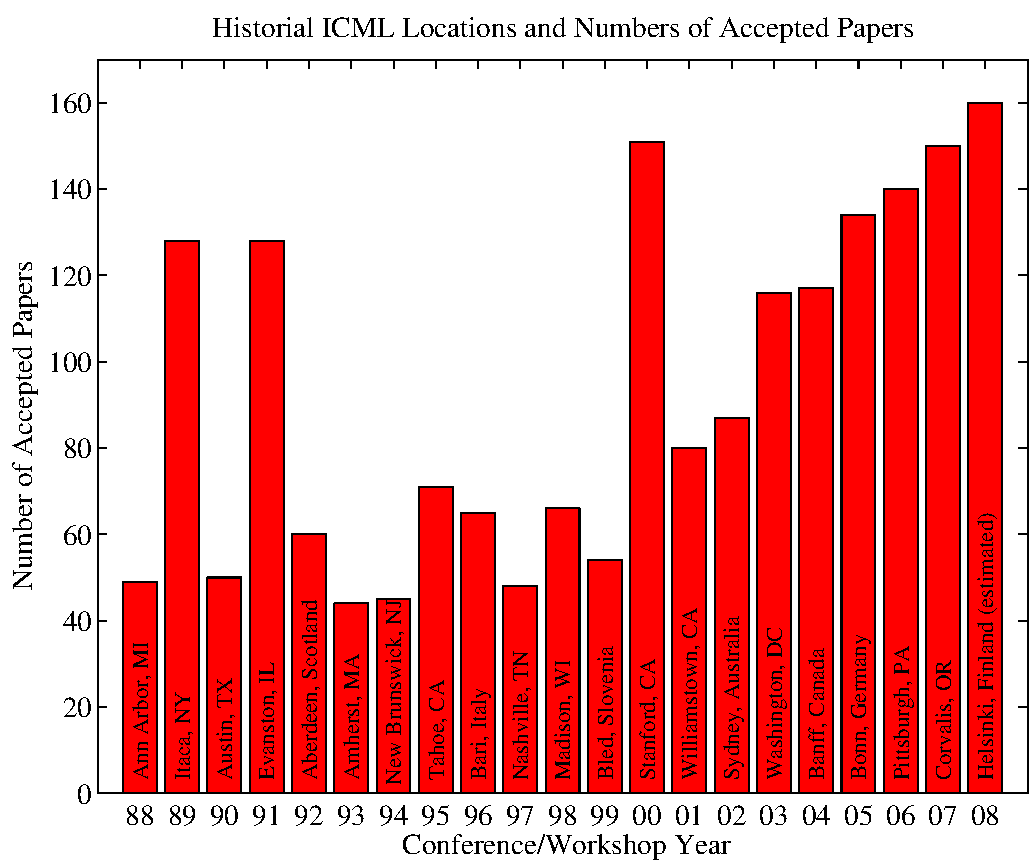
\includegraphics[width=\columnwidth]{icml2015stylefiles/icml_numpapers}}
\caption{An example of a training schedule optimized by hyper-gradient descent.}
\label{fig:optimal schedule}
\end{center}
\vskip -0.2in
\end{figure} 

\begin{figure}[ht]
\vskip 0.2in
\begin{center}
%\centerline{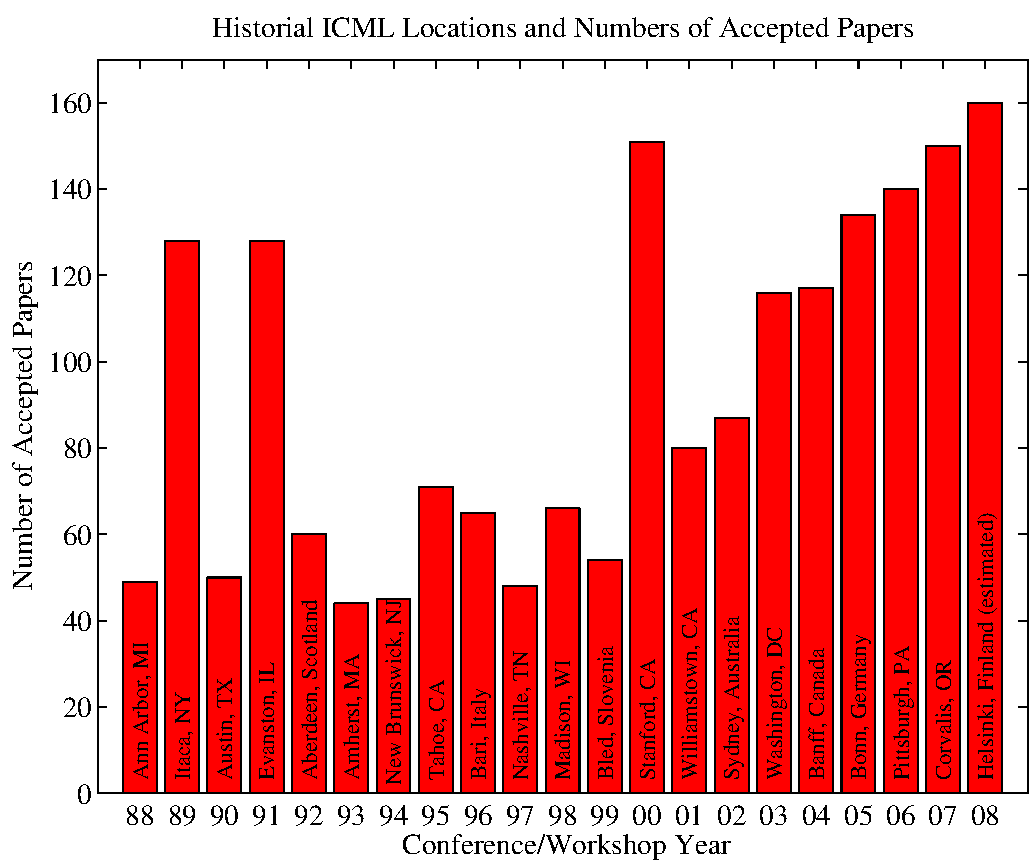
\includegraphics[width=\columnwidth]{icml2015stylefiles/icml_numpapers}}
\caption{An example of an initial weight distribution optimized by hyper-gradient descent.}
\label{fig:optimal schedule}
\end{center}
\vskip -0.2in
\end{figure} 


\section{Conclusion}

Implementing reversible learning as presented in this paper requires either that the learning algorithm is a form of (stochastic) gradient descent with

\section*{Acknowledgments} 


\bibliography{references.bib}
\bibliographystyle{icml2015stylefiles/icml2015}

\end{document} 

